% This section might vary depending on the field of research. Consider this the approach, design, or architecture of the proposed system. You can also include implementation if it applies to your research.

% Include at least one figure. Figure that shows the architecture of the proposed system, concepts of the proposed algorithm, etc. One figure that you could put into a slide that tells your idea. 

% figure needed for displaying the architecture so matlab to riscv

% Include actual implementation details. 
% Describe the implementation language, platform, location, and dependencies on the packages.

The objective of this research is the architecture and implementation of a cohesive, automated compilation pipeline capable of translating high-level algorithms into low-level optimized silicon instructions. This section details the system architecture, focusing on the transformation mechanisms, the categorization of vectorizable workloads, and the underlying platform dependencies. 

The compiler pipeline is implemented as a continuous, directed data flow that isolates high-level semantic analysis from low-level hardware optimizations. The system architecture can be visualized through a structured sequence of state transitions and module interactions in Figure 3.1. The pipeline starts by taking in raw .m files authored by clinical researchers. These files contain standard MATLAB syntax, incorporating dynamic array allocations, calls to proprietary signal processing toolboxes, and high-level, implicitly parallel matrix arithmetic.

\begin{figure}[h]
    \centering
    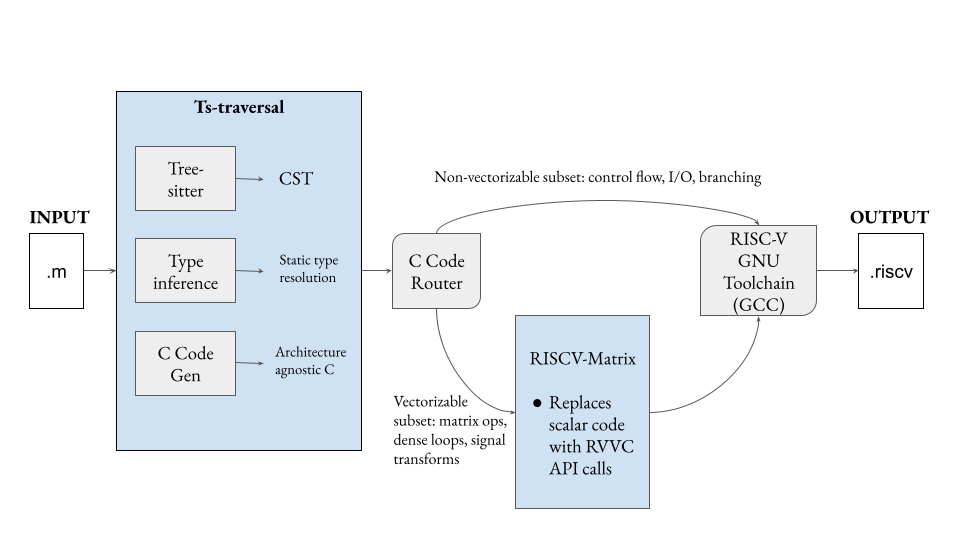
\includegraphics[width=\textwidth]{figs/pipeline_architecture1.png}
    \caption{System architecture of the MATLAB-to-RISC-V compilation pipeline. Raw \texttt{.m} files are parsed and type-inferred by the ts-traversal engine (Stage 1), then routed: vectorizable operations are mapped to RVV intrinsics via the RISCV-Matrix library (Stage 2), while non-vectorizable code passes through unmodified. Both subsets are merged by the RISC-V GCC toolchain into a single binary, validated on the Spike ISA simulator.}
    \label{fig:pipeline-architecture}
\end{figure}


These raw files are passed into the first major component of the pipeline, the ts-traversal engine \cite{ts}. This engine executes a multi-phase transformation. First, it uses the TreeSitter and TreeSitter-Matlab parsing libraries to generate a concrete syntax tree (CST). This representation captures the complete syntactic structure of the input algorithms. The engine must thus perform rigorous type inference on the dynamically typed input MATLAB code. The inference algorithms in ts-traversal then traverse the CST to deduce the maximal dimensions, memory allocation requirements, and fundamental data types of all variables, mapping them to statically typed C constructs. The output of this initial phase is standard C code. At this point in the pipeline, the semantic intent of the MATLAB script is entirely preserved. Still, the resulting C code remains architecturally agnostic and relies on standard, scalar loop iterations. 

To implement the necessary hardware optimizations, the pipeline will employ an internal routing system.
The generated C code consists of two distinct computational subsets. The non-vectorizable subset comprises complex control-flow logic, sequential input/output operations, and highly divergent branching structures. Conversely, the vectorizable subset encompasses large-scale loops, dense matrix arithmetic, and parallelizable signal transformations. The routing mechanism will isolate this vectorizable subset and direct it to the second major component of the pipeline, the RISC-V Matrix library \cite{riscvmatrix}.

% Note about the above paragraph: this is how I am assuming I will have to combine the two repos. Subject to change.

Within the RISCV-Matrix library, the standard scalar loops generated by the previous step are systematically replaced by API calls mapped to the library's headers. These headers contain highly optimized, inline RVV C intrinsics. This transformation effectively converts the vectorizable subset into heavily accelerated C code explicitly built for the parallel execution capabilities of HALO's microcontroller.

The final phase of the architectural model involves compiling and deploying the codebase. Both the unmodified non-vectorizable subset and the vectorized subset are passed into the RISC-V GNU Compiler toolchain. The compiler merges these subsets and statically links the optimized vector library to produce a highly efficient RISC-V binary. Thus, the pipeline generates an executable containing the exact algorithms authored by neuroscientists in Matlab while meeting the power and latency requirements of the implanted chip. 

The validation, execution modeling, and accurate instruction-level benchmarking of the generated binaries are conducted using the Spike ISA simulator, since the actual HALO silicon is not readily available. Spike provides a fully functional, instruction-accurate model of a RISC-V core with the RVV extension, enabling precise tracking of executed instructions, vector register utilization, and overall execution cycles. This enables the continuous, iterative refinement of both the source-to-source compiler and the vectorization library without requiring constant access to the physical test hardware. To bridge the TypeScript translation engine and the C-based vectorization, a unified build system is currently under development to automate the entire data flow from source ingestion to simulator execution via a single command-line interface.